\documentclass{article}
\usepackage{graphicx}
\usepackage{amsmath}
\usepackage{amsfonts}
\usepackage{amssymb}
\begin{document}
	\author{Hu Xiping}
	\title{Note on Mathematica Programming}
	\maketitle
	\section{Basic Usage of Wolfram Language}
		\paragraph{Evaluating Commands}
			On desktop and web, you may press \textbf{Shift}+\textbf{Enter}. On mobile, press the Wolfram icon button
		\paragraph{Auto Complete}
			Within the Mathematica notebook, you'll see a variety of aids to help you enter the Wolfram Language.
		\paragraph{Studying Resources}
			You may RTFM(Read The F***ing Manual) or visit Wolfram website to equip essential skills on Wolfram Language. Or you can JFGI(Just F***ing Google It) if your problem can't be solved. Note that you need to use Google instead of Baidu due to study efficiency and you'd better use English to search for help.
			
		\section{Elementary Arithmetic}
			\begin{tabular}{|c|c|c|}
				\hline 
				Command & Expression & Example \\ 
				\hline 
				Add & + & 2+2 \\ 
				\hline
				Subtract & - & 2-2 \\ 
				\hline
				Multiply & * & 2*2 \\ 
				\hline
				Division & / & 2/2 \\ 
				\hline
				Power & \^{} & 2\^{}2 \\ 
				\hline
				Brackets & ( and ) & (2+3)/5 \\
				\hline
			\end{tabular} 
		\section{Introduction to Functions}
			\paragraph{Example}
				Plus[3, 4, 5] 
			\paragraph{Usage}
				Functions names are all started with capital letters. To use a function, attach a "[]" behind the name of function and input parameters separated with "," into the brackets. Tip: insert a single space after the comma to make your code more visualized.
			\paragraph{Another Example}
				Times[2, Plus[2, 3]]
			\paragraph{Usage}
				You may use the output of function as a parameter of other functions.
			\subsection{Some basic functions}
				Plus[2, 3],
				Subtract[2, 3],
				Times[2, 3],
				Divide[2, 3],
				Power[2, 3],
				Max[2, 3],
				Min[2, 3],
				RandomInteger[100]
		\section{Introduction to Lists}
			\paragraph{List is a way to store numbers} \{1,2,3,4,5\} is a list
			\paragraph{Range[] is a function to create lists}
			\begin{figure}[h!]
				\centering
				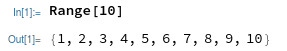
\includegraphics[width=0.7\linewidth]{pics/Range}
				\caption{Function Range[]}
				\label{fig:range}
			\end{figure}
			\paragraph{Reverse[] is a function to reverse the elements in a list}
			\begin{figure}[h!]
				\centering
				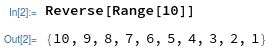
\includegraphics[width=0.7\linewidth]{pics/Reverse}
				\caption{Function Reverse[]}
				\label{fig:reverse}
			\end{figure}
			\paragraph{Use Join[] to join Lists together}
			\begin{figure}[h!]
				\centering
				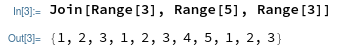
\includegraphics[width=0.7\linewidth]{pics/Join}
				\caption{Function Join[]}
				\label{fig:join}
			\end{figure}
		\section{Visualizing Lists}
		
		
		
			
			
			
			
				
				
\end{document}